\subsection{Scadenze}
\begin{itemize}
\setlength\itemsep{0em}
    \item RTB (Requirements and Technology Baseline) : 2024-06-07;
    \item PB (Product Baseline) : 2024-07-26;
    \item CA (Customer Acceptance) : 2024-08-09.
\end{itemize}
\subsection{Verso la RTB}
\textit{Periodo: dal 2024-04-01 al 2024-06-07}
\newpage
\subsubsection{Primo periodo}
\textit{Periodo: dal 2024-04-01 al 2024-04-19}
\\\\
Nella fase iniziale, assume prioritaria importanza la discussione di tutte le regole precedentemente adottate e implementate nel corso del progetto, ma che non sono ancora state formalizzate mediante documentazione. Questo processo mira a produrre un documento scritto accessibile a tutti i membri del team, al fine di dissipare eventuali ambiguità riguardo l'esecuzione delle attività e l'utilizzo delle risorse.
\\
Inoltre, durante questa fase, è cruciale identificare tutti i potenziali rischi che potrebbero ostacolare il progresso del progetto, al fine di prevenirli e non essere colti impreparati. Un'altra priorità consiste nell'avviare la pianificazione delle prime attività e delle relative milestone, al fine di organizzare le risorse disponibili e fornire una stima preventiva dei tempi e dei costi.
\\
\begin{figure}[h]
    \centering
    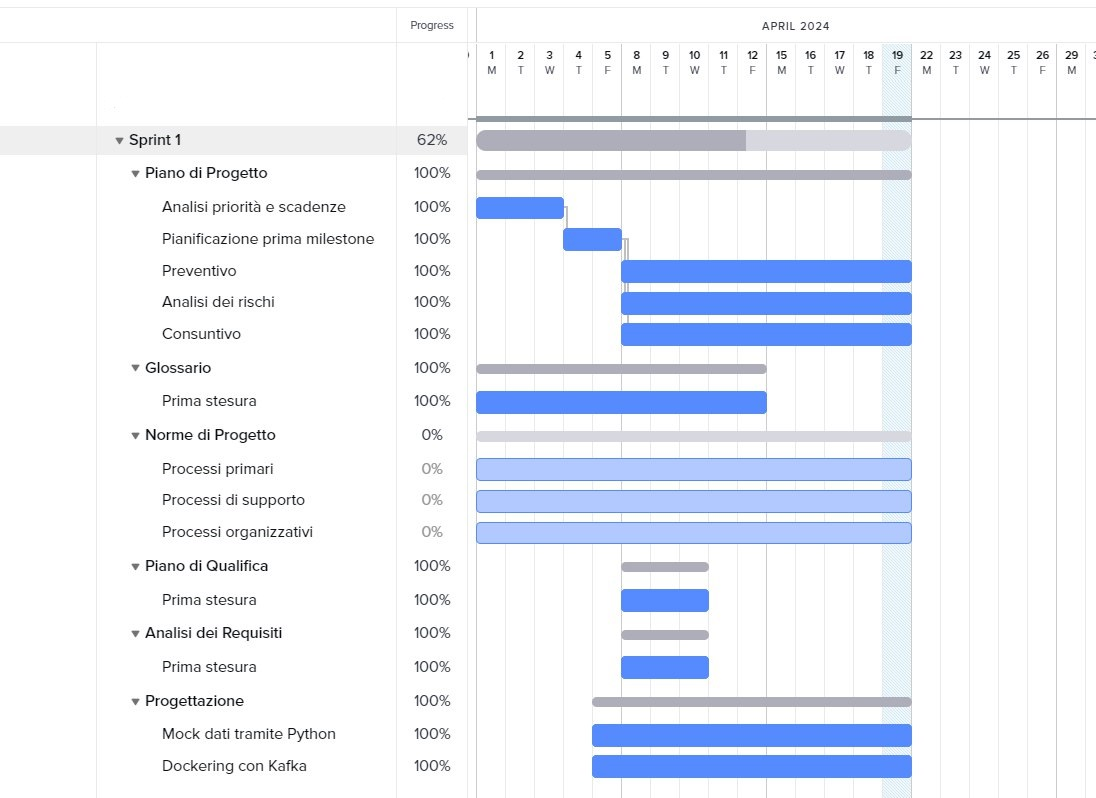
\includegraphics[width=15cm]{./asset/gantt1.jpeg}
    \caption{Diagramma di Gantt rappresentativo del primo periodo}
    \label{figure:Diagramma di Gantt rappresentativo del primo periodo}
\end{figure}
\subsubsection{Secondo periodo}
\textit{Periodo: dal 2024-04-22 al 2024-05-03}
\\\\
In questa fase del processo, assume un'importanza fondamentale condurre un'analisi dettagliata del capitolato al fine di identificare accuratamente i casi d'uso necessari. Inoltre, al fine di evitare ambiguità e decisioni errate, si raccomanda di organizzare uno o più incontri con il proponente per condividere le idee e risolvere i dubbi emersi durante l'analisi, che sarà notevolmente più approfondita rispetto a quella svolta durante la selezione del capitolato.
Da questo processo di analisi, si darà inizio alla stesura dell'\textit{Analisi dei Requisiti}, un documento di vitale importanza per il progetto poiché conterrà tutti i casi d'uso individuati, nonché i requisiti obbligatori, desiderabili e opzionali.
È altresì consigliabile redigere il \textit{Piano di Qualifica} in questa fase, il quale sarà fondamentale per definire i metodi volti a garantire la qualità dei processi e dei prodotti nel corso dello svilupppo.

\subsubsection{Terzo periodo}
\textit{Periodo: dal 2024-04-29 al 2024-05-17}
Con la completamento dell'\textit{Analisi dei Requisiti}, assume un ruolo cruciale l'approfondimento delle tecnologie e degli strumenti necessari per l'implementazione del prodotto. Questo processo consentirà la realizzazione del \textit{PoC} (Proof of Concept), una versione semplificata del prodotto finale che mira a fornire indicazioni sulla validità della direzione intrapresa e a dimostrare al committente la correttezza dell'approccio di sviluppo.

\subsubsection{Quarto periodo}
\textit{Periodo: dal 2024-05-20 al 2024-06-07}
\\\\
In questa fase conclusiva del processo, assume primaria importanza sia la progettazione che l'effettiva implementazione del \textit{PoC}. Parallelamente, diventa imprescindibile il perfezionamento e la verifica finale dei documenti in vista della revisione pianificata per l'inizio del mese di giugno.

\subsection{Verso la PB}
\textit{Periodo: dal 2024-06-08 al 2024-07-26}
\\\\
Superata la prima revisione, l'obiettivo principale è realizzare una prima versione del prodotto finale che dimostri come ha già fatto il \textit{PoC}, nella sua semplicità, 
che requisiti e tecnologie scelte possono coesistere nello stesso prodotto. 
\\
Sarà, quindi, fondamentale la progettazione per arrivare ad avere un design che sia quello definitivo e poi avere un avanzamento consistente di codifica e verifica.

\subsection{Verso la CA}
\textit{Periodo: 2024-07-26 - 2024-08-09}
\\\\
Superata la seconda revisione, l'obiettivo rimane quello di presentare al proponente il prodotto finale.